\chapter{Ergebnisse}
\label{ch:Ergebnisse}

\section{Modellauswahl und Detektorkalibrierung}

Tabelle~\ref{tab:forecaster_selection} zeigt die auf dem Tuningabschnitt
ermittelten Werte der beiden LSTM-Konfigurationen. Der Mittelwert der beiden
relativen MAE-Werte dient ausschließlich der Modellauswahl.

\begin{table}[htb]
  \centering
  \caption{Ergebnis der LSTM-Auswahl auf dem Tuningabschnitt. Eigene
    Darstellung.}
  \label{tab:forecaster_selection}
  \begin{tabular}{lrrrr}
    \hline
    Modell & beste Epoche & MAE Visitors & MAE Duration & mittl. rel. MAE \\
    \hline
    Small & 32 & 16{,}400 & 3{,}486 & 0{,}883 \\
    Regularized & 21 & 15{,}176 & 3{,}598 & 0{,}851 \\
    \hline
  \end{tabular}
\end{table}

Gewählt wird die regularisierte Konfiguration mit 64 LSTM-Einheiten, einer
dichten Schicht mit 48 Einheiten, einem sechsdimensionalen Sensor-Embedding,
Dropout 0{,}25 und einer Lernrate von 0{,}0005. Der Trainingsverlauf ist in
Abbildung~\ref{fig:forecaster_training} dargestellt.

\begin{figure}[htb]
  \centering
  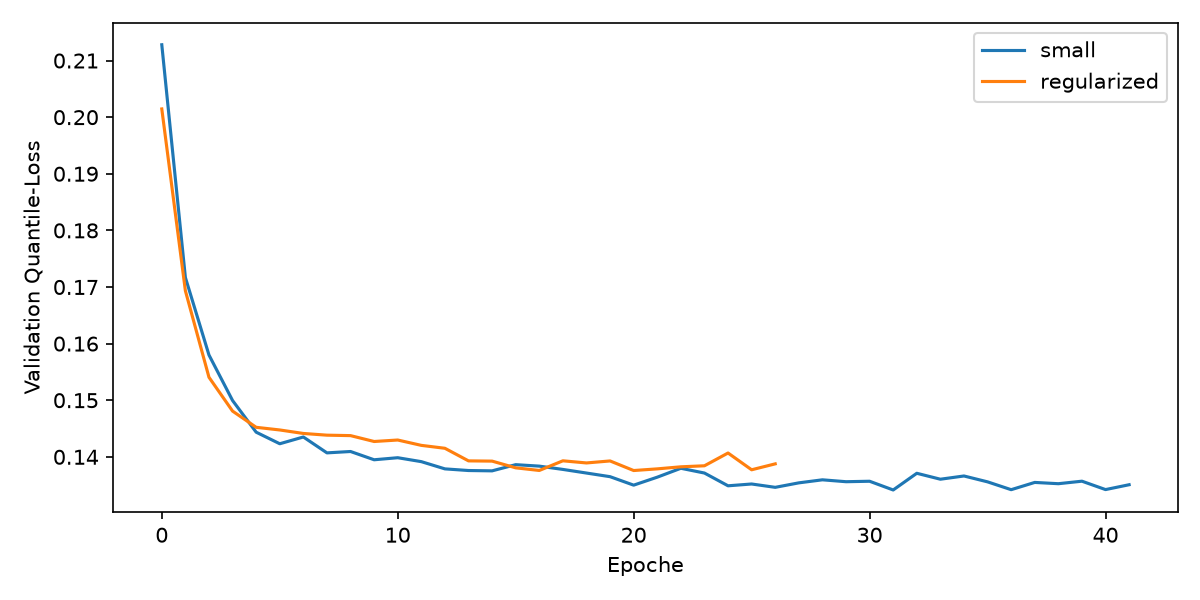
\includegraphics[width=0.82\textwidth]{../saved_models/forecaster/training_history.png}
  \caption{Validierungs-Pinball-Loss der beiden Modellkandidaten. Eigene
    Darstellung.}
  \label{fig:forecaster_training}
\end{figure}

Die gemeinsame empirische 1-\%-Schwelle beträgt 0{,}7486. Unter den 15
zulässigen Alarmregeln wählt die Kalibrierung zusätzlich die Bedingung, dass
mindestens drei der letzten vier lückenlosen Messscores den niedrigeren Wert
0{,}3082 überschreiten. Auf den unveränderten 368 Kalibrierungspunkten erzeugt
diese Regel zwei Alarme beziehungsweise 0{,}54~\% und hält damit das vorab
festgelegte 1-\%-Budget ein. Der Macro-Ereignis-F1 der
Kalibrierungsinjektionen beträgt 0{,}746. Dieser Wert ist ein Auswahlkriterium
und kein Testergebnis.

\section{Prognosegüte im Testabschnitt}

\begin{table}[htb]
  \centering
  \caption{Prognosegüte auf 1.346 gemessenen Testzielen. Die Abdeckung und
    Breite beziehen sich auf die empirisch kalibrierten Intervalle. Eigene
    Darstellung.}
  \label{tab:forecaster_forecast_results}
  \begin{tabular}{lrrrrrr}
    \hline
    Ziel & MAE & RMSE & MASE & rel. MAE & Abdeckung & Breite \\
    \hline
    Visitors & 12{,}114 & 22{,}962 & 0{,}622 & 0{,}745 & 99{,}63~\% & 224{,}99 \\
    AvgDuration & 4{,}124 & 7{,}540 & 0{,}855 & 0{,}821 & 99{,}55~\% & 98{,}54 \\
    \hline
  \end{tabular}
\end{table}

Beide MASE-Werte und beide relativen Test-MAE-Werte liegen unter eins. Die
Medianprognose ist damit im Mittel genauer als die jeweils verwendete
saisonale Skalierung beziehungsweise $t-24$-Testbaseline. Die gemeinsame
empirische Abdeckung beider Zielgrößen beträgt 99{,}26~\%. Gleichzeitig sind
die Intervalle insbesondere für die Passantenzahl breit. Die hohe Abdeckung
ist deshalb zusammen mit der Breite zu interpretieren und belegt allein keine
hohe Trennschärfe des Anomaliedetektors.

\section{Kandidaten im unveränderten Datensatz}

Die eingefrorene Hybridregel markiert 15 der 1.346 gemessenen Testpunkte. Sie
bilden elf zusammenhängende Forecast-Ereignisse. Die ursprüngliche reine
1-\%-Punktschwelle hätte zehn Punkte markiert; die Persistenzregel ergänzt somit
fünf moderate Punkte. Abbildung~\ref{fig:forecaster_example} zeigt den Sensor
mit den meisten Forecast-Kandidaten. Die rote Markierung bedeutet eine
statistische Abweichung und keine fachlich bestätigte Anomalie.

\begin{figure}[htb]
  \centering
  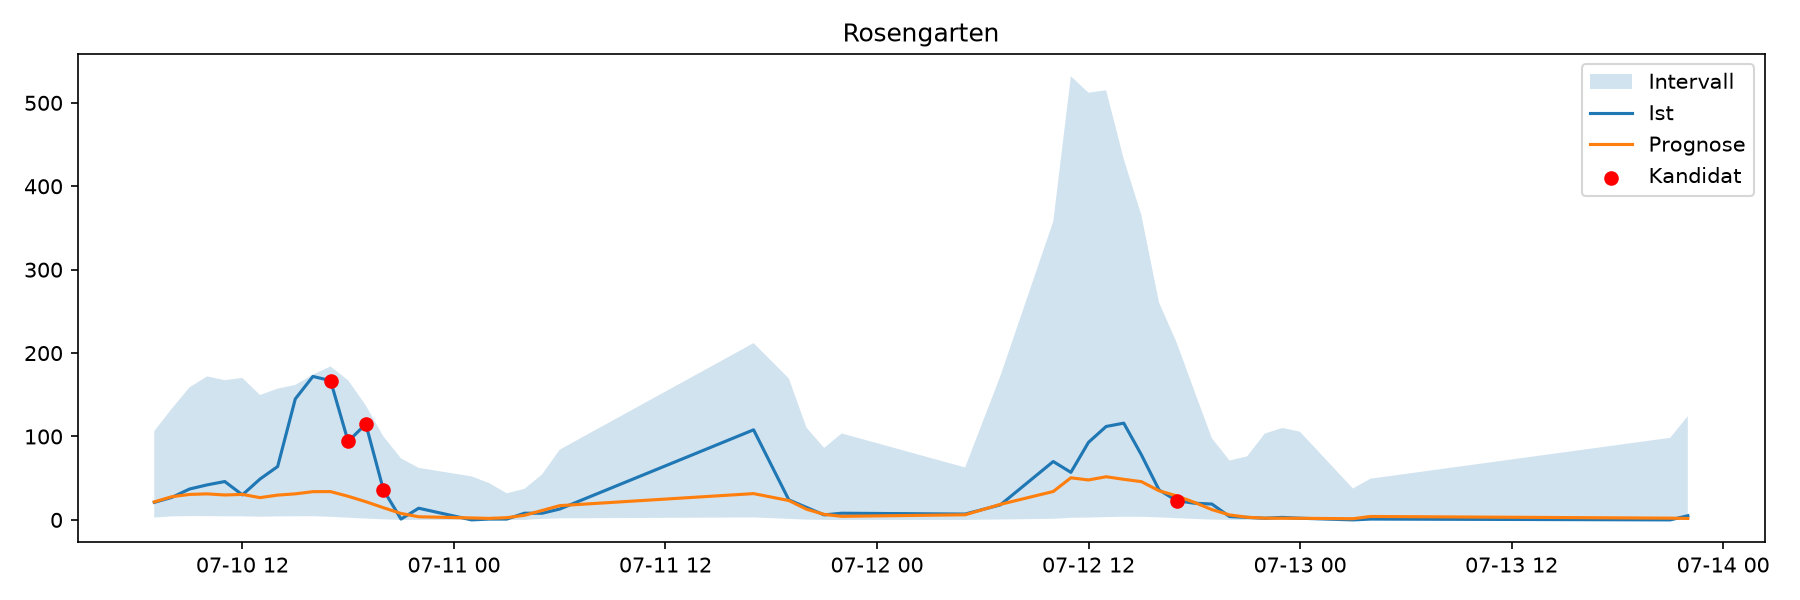
\includegraphics[width=\textwidth]{../saved_models/forecaster/anomalies_example.png}
  \caption{Messung, Medianprognose, empirisch kalibriertes Intervall und
    Forecast-Kandidaten eines Beispielsensors. Eigene Darstellung.}
  \label{fig:forecaster_example}
\end{figure}

Zusätzlich besitzen 1.333 Testziele keine Originalmessung. Diese werden zu 275
zusammenhängenden Datenlücken-Ereignissen gruppiert und separat ausgewiesen.
Sie sind Hinweise auf fehlende Sensordaten, aber nicht automatisch Anomalien
des Passantenverhaltens. Werden Forecast- und Datenqualitätsalarme gemeinsam
gruppiert, entstehen 282 Ereignisse; diese Zahl darf daher nicht als Anzahl
erkannter Verhaltensanomalien interpretiert werden.

\section{Ergebnisse der Anomalieinjektion}

Tabelle~\ref{tab:forecaster_injection_results} fasst die starken Injektionen
der Stärke 2{,}0 und den gefilterten sechs Stunden langen Stuck-at-Test über
drei Testseeds zusammen. Die Referenzspalten zeigen die unveränderte reine
1-\%-Punktschwelle. Sämtliche Treffer sind inkrementell gegenüber dem jeweils
gepaarten unveränderten Lauf.

\begin{table}[htb]
  \centering
  \small
  \caption{Punkt- und Ereignisergebnisse der Testinjektionen. R = Recall,
    Ref. = Referenzdetektor. Eigene Darstellung.}
  \label{tab:forecaster_injection_results}
  \begin{tabular}{lrrrrrr}
    \hline
    Typ & Punkt-R & Punkt-F1 & Ereignis-R & Ereignis-F1 & Ref.-R & Ref.-F1 \\
    \hline
    Spike, 2{,}0 & 0{,}633 & 0{,}732 & 0{,}633 & 0{,}767 & 0{,}633 & 0{,}775 \\
    Dip, 2{,}0 & 0{,}533 & 0{,}651 & 0{,}533 & 0{,}658 & 0{,}533 & 0{,}672 \\
    Level-Shift, 2{,}0 & 0{,}708 & 0{,}742 & 0{,}861 & 0{,}878 & 0{,}833 & 0{,}883 \\
    Drift, 2{,}0 & 0{,}458 & 0{,}543 & 0{,}750 & 0{,}810 & 0{,}694 & 0{,}780 \\
    Stuck-at, 6 h & 0{,}237 & 0{,}345 & 0{,}371 & 0{,}499 & 0{,}315 & 0{,}404 \\
    \hline
  \end{tabular}
\end{table}

Die Persistenzregel erhöht den Ereignis-Recall erwartungsgemäß bei
mehrstündigen Veränderungen: bei starkem Level-Shift von 0{,}833 auf 0{,}861,
bei starkem Drift von 0{,}694 auf 0{,}750 und bei Stuck-at von 0{,}315 auf
0{,}371. Für einstündige Spikes und Dips entsteht kein Recall-Gewinn. Bei
Level-Shift und den punktuellen Typen sinkt der Ereignis-F1 geringfügig, weil
zusätzliche Alarme die Precision belasten. Die Regel verbessert somit nicht
jede einzelne Kennzahl, erhöht aber gezielt die Sensitivität für anhaltende
Abweichungen, ohne die empirische Kalibrierungs-Alarmrate zu erhöhen.

Schwache Injektionen bleiben schwierig. Bei Stärke 0{,}5 beträgt der
Ereignis-Recall 0{,}067 für Spike, 0{,}017 für Dip, 0{,}167 für Level-Shift
und 0{,}028 für Drift. Der Detektor erkennt folglich nicht jede definierte
Anomalie. Die vollständigen Werte aller Stärken einschließlich Precision,
PR-AUC, IoU und Verzögerung stehen in
\texttt{injection\_benchmark.csv} und
\texttt{injection\_benchmark.json}.

\section{Diskussion und Limitationen}

Die Ergebnisse beantworten die Forschungsfrage differenziert. Der globale
Quantil-Forecaster übertrifft die saisonale Baseline im mittleren
Prognosefehler. Starke punktuelle und mehrstündige Injektionen werden teilweise
bis überwiegend erkannt; die zusätzliche Persistenz verbessert vor allem
Level-Shift, Drift und Stuck-at. Für schwache Anomalien und einzelne Dips ist
die Sensitivität gering.

Die synthetische Ground Truth gilt ausschließlich für die definierten
Transformationen. Sie belegt weder den Recall unbekannter realer Anomalien noch
die fachliche Richtigkeit der elf Kandidaten im Originaldatensatz. Der nur zwei
Wochen umfassende Datensatz begrenzt außerdem die beobachtbaren Wochenmuster
und die Größe von Tuning und Kalibrierung. Zeitliche Abhängigkeit verhindert
eine klassische verteilungsfreie Conformal-Garantie. Schließlich wurde der
Testzeitraum im Verlauf der retrospektiven Entwicklung bereits betrachtet;
die Testinjektionen sind durch neue Seeds und eine eingefrorene Regel getrennt,
stellen aber keine vollständig unangetastete konfirmatorische Studie dar.
